%%%%%%%%%%%%%%%%%%%%%%%%%%%%%%%%%%%%%%%%%%%%%%%%%%%%%%%%%%%%%%%%%%%%%%
\subsection{\label{sec:Contrib-CondorView-Install}
Installing CondorView Contrib Modules}
%%%%%%%%%%%%%%%%%%%%%%%%%%%%%%%%%%%%%%%%%%%%%%%%%%%%%%%%%%%%%%%%%%%%%%

% Need a short description of CondorView and why
% it might be wanted.

\index{CondorView}
\index{installation!CondorView contrib module}
To install CondorView for your pool, you really need two things:
\begin{enumerate}
\item The CondorView server, which collects historical information.
\item The CondorView client, a Java applet that views this data.
\end{enumerate}

These are separate modules, and they are installed separately.

%%%%%%%%%%%%%%%%%%%%%%%%%%%%%%%%%%%%%%%%%%%%%%%%%%%%%%%%%%%%%%%%%%%%%%
\subsection{\label{sec:CondorView-Server-Install}
Installing the CondorView Server Module}
%%%%%%%%%%%%%%%%%%%%%%%%%%%%%%%%%%%%%%%%%%%%%%%%%%%%%%%%%%%%%%%%%%%%%%

The CondorView server is an enhanced version of the
\Condor{collector}
\index{CondorView}
that logs information on disk, providing a 
persistent, historical database of your pool state.
This includes machine state, as well as the state of jobs submitted by
users, and so on.
This enhanced \Condor{collector} is the version 6.1 development
series, but it can be installed in a 6.0 pool.
The historical information logging can be turned on or off, so you can
install the CondorView collector without using up disk space for
historical information if you don't want it.

To install the CondorView server, you download the appropriate
binary module for the platform on which you will run CondorView.
This does not have to be the same platform as your existing central
manager (see below).
After you uncompress and untar the module, you will have a directory
with a \File{view\_server.tar} file, a \File{README}, and so on.
The \File{view\_server.tar} acts much like the \File{release.tar} file
for a main release of Condor.
It contains all the binaries and supporting files you would install in
your release directory:
\begin{verbatim}
        sbin/condor_collector
        etc/examples/condor_config.local.view_server
\end{verbatim}

You have two options to choose from when deciding how to install this
enhanced \Condor{collector} in your pool:
\begin{enumerate}
\item Replace your existing \Condor{collector} and use the new
version for both historical information and the regular role the 
collector plays in your pool.
\item Install the new \Condor{collector} and run it on a separate host
from your main \Condor{collector} and configure your machines to send
updates to both collectors.
\end{enumerate}

If you replace your existing collector with the enhanced version,
there may be bugs or problems that
cause problems for your pool.
This is because it is development code.
Installing the enhanced version on a separate
host may cause problems, but only CondorView will be affected, not
your entire pool.
Unfortunately, installing the CondorView collector on a separate host
generates more network traffic (from all the duplicate updates that
are sent from each machine in your pool to both collectors).
In addition, the installation procedure to have both collectors
running is a more complicated process.
Decide for yourself which solution you feel more
comfortable with.

What follows are details common to both types of installation.

%%%%%%%%%%%%%%%%%%%%%%%%%%%%%%%%%%%%%%%%%%%%%%%%%%%%%%%%%%%%%%%%%%%%%%
\subsubsection{\label{sec:CondorView-Server-Setup}
Setting up the CondorView Server Module} 
%%%%%%%%%%%%%%%%%%%%%%%%%%%%%%%%%%%%%%%%%%%%%%%%%%%%%%%%%%%%%%%%%%%%%%

\index{CondorView!installation|(}
Before you install the CondorView collector (as described in the
following sections), you have to add a few settings to the local
configuration file of that machine to enable historical data collection.
These settings are described in detail in the Condor Version 6.1
Administrator's Manual, in the section ``\condor{collector} Config File
Entries''.
A short explanation of the entries you must customize is
provided below. 
These entries are also explained in the
\File{etc/examples/condor\_config.local.view\_server} file, included
in the contrib module.
Insert that file into the local configuration file for your
CondorView collector host and customize as appropriate at your site.  

\begin{description}

\item[\Macro{POOL\_HISTORY\_DIR}] This is the directory where
historical data will be stored.
This directory must be writable by whatever user the CondorView
collector is running as (usually the user condor).  
There is a configurable limit to the maximum space required for all
the files created by the CondorView server called
(\Macro{POOL\_HISTORY\_MAX\_STORAGE}). 

\Note This directory should be separate and different from the
\File{spool} or \File{log} directories already set up for
Condor.
There are a few problems putting these files into either of those
directories.

\item[\Macro{KEEP\_POOL\_HISTORY}] This is a boolean value that determines
if the CondorView collector should store the historical information.
It is false by default, which is why you must specify it as true in
your local configuration file to enable data collection.

\end{description}

Once these settings are in place in the local configuration file for your
CondorView server host, you must to create the directory you specified
in \Macro{POOL\_HISTORY\_DIR} and make it writable by the user your
CondorView collector is running as.
This is the same user that owns the \File{CollectorLog} file in
your \File{log} directory. The user is usually condor.

Once these steps are completed, you are ready to install the new
binaries and you will begin collecting historical information.
After that, install the CondorView client contrib module which
contains the tools used to query and display this information.

%%%%%%%%%%%%%%%%%%%%%%%%%%%%%%%%%%%%%%%%%%%%%%%%%%%%%%%%%%%%%%%%%%%%%%
\subsubsection{\label{sec:CondorView-Server-Only}
CondorView Collector as Your Only Collector} 
%%%%%%%%%%%%%%%%%%%%%%%%%%%%%%%%%%%%%%%%%%%%%%%%%%%%%%%%%%%%%%%%%%%%%%

To install the new CondorView collector as your main collector, you
replace your existing binary with the new one, found in
the \File{view\_server.tar} file.
Move your existing \File{\condor{collector}}
binary out of the way with the \Prog{mv} command.
For example:
\begin{verbatim}
        % cd /full/path/to/your/release/directory
        % cd sbin
        % mv condor_collector condor_collector.old
\end{verbatim}
Then, from that same directory, untar the
\File{view\_server.tar} file into your release directory.
This will
install a new \File{\condor{collector}} binary and an example
configuration file.
Within 5 minutes, the \Condor{master} will notice the new timestamp on
your new \File{\condor{collector}} binary, shutdown your existing
collector, and spawn the new version.
You will see messages about this in the log file for your
\Condor{master} (usually \File{MasterLog} in your \File{log}
directory).
Once the new collector is running, it is safe to remove the old
binary, although you may want to keep it around in case you have
problems with the new version and want to revert back.

Once this is completed, add configuration file entries
to the local configuration file on your central manager to enable historical
data collection as
described below in the ``Configuring the CondorView Server 
Module'' section.

%%%%%%%%%%%%%%%%%%%%%%%%%%%%%%%%%%%%%%%%%%%%%%%%%%%%%%%%%%%%%%%%%%%%%%
\subsubsection{\label{sec:CondorView-Server-Both}
CondorView Collector in Addition to Your Main Collector} 
%%%%%%%%%%%%%%%%%%%%%%%%%%%%%%%%%%%%%%%%%%%%%%%%%%%%%%%%%%%%%%%%%%%%%%

Installing the CondorView collector in addition to your regular
collector requires a little extra work.
First, untar the \File{view\_server.tar} file into a
temporary location (not your main release directory).
Copy the \File{sbin/\condor{collector}} file from the temporary location
to your main release directory's sbin with a new name (such as
\File{\condor{collector}.view\_server}).

Next, configure whatever host is going to run your separate
CondorView server to spawn this new collector in addition to
other daemons it is running.
You do this by adding \Expr{COLLECTOR} to the \Macro{DAEMON\_LIST} on
this machine and defining what \Expr{COLLECTOR} means.
For example:
\begin{verbatim}
        DAEMON_LIST = MASTER, STARTD, SCHEDD, COLLECTOR
        COLLECTOR = $(SBIN)/condor_collector.view_server
\end{verbatim}
For this change to take effect, you must re-start the
\Condor{master} on this host (which you can do with the
\Condor{restart} command, if you run the command from a machine with 
administrator access to your pool.
(See section~\ref{sec:Host-Security} on
page~\pageref{sec:Host-Security} for full details of IP/host-based
security in Condor).

As a last step, you tell all the machines in your pool to start sending
updates to both collectors.
You do this by specifying the following setting in your global
configuration file:
\begin{verbatim}
        CONDOR_VIEW_HOST = full.hostname
\end{verbatim}
where \verb@full.hostname@ is the full hostname of the machine where you
are running your CondorView collector.

Once this setting is in place, send a
\Condor{reconfig} to all machines in your pool so the changes take
effect.
This is described in section~\ref{sec:Reconfigure-Pool} on
page~\pageref{sec:Reconfigure-Pool}.

%%%%%%%%%%%%%%%%%%%%%%%%%%%%%%%%%%%%%%%%%%%%%%%%%%%%%%%%%%%%%%%%%%%%%%
\subsection{\label{sec:CondorView-Client-Install}
Installing the CondorView Client Contrib Module} 
%%%%%%%%%%%%%%%%%%%%%%%%%%%%%%%%%%%%%%%%%%%%%%%%%%%%%%%%%%%%%%%%%%%%%%

% We refer to the make_stats program often in this section; make a
% macro for it.
\newcommand{\MakeStats}{\Prog{make\_stats}}

The CondorView Client contrib module is used to automatically generate
World Wide Web (WWW) pages displaying usage statistics of your Condor
Pool.
Included in the module is a shell script which invokes the \Condor{stats}
command to retrieve pool usage statistics from the CondorView server and
generate HTML pages from the results.  
Also included is a Java applet which graphically visualizes Condor 
usage information.  
Users can interact with the applet to customize the visualization and to
zoom in to a specific time frame.
Figure~\ref{fig:view-screenshot} on page~\pageref{fig:view-screenshot}
is a screenshot of a web page created by CondorView.  
To get a further feel for what pages generated by CondorView look like,
you can view the statistics for the University of Wisconsin-Madison pool
by going to URL \Url{http://www.cs.wisc.edu/condor} and clicking on
Condor View.

\begin{figure}[hbt]
\centering
\includegraphics{admin-man/view-screenshot.ps}
\caption{\label{fig:view-screenshot}Screenshot of CondorView Client}
\end{figure}

After unpacking and installing the CondorView Client, a script named
\MakeStats\ can be invoked to create HTML pages displaying Condor usage
for the past hour, day, week, or month.  
By using the Unix \Prog{cron} facility to periodically execute
\MakeStats, Condor pool usage statistics can be kept up to date
automatically.  
This simple model allows the CondorView Client to be easily installed;
no Web server CGI interface is needed.

%%%%%%%%%%%%%%%%%%%%%%%%%%%%%%%%%%%%%%%%%%%%%%%%%%%%%%%%%%%%%%%%%%%%%%
\subsubsection{\label{sec:condorview-client-step-by-step}
Step-by-Step Installation of the CondorView Client}
%%%%%%%%%%%%%%%%%%%%%%%%%%%%%%%%%%%%%%%%%%%%%%%%%%%%%%%%%%%%%%%%%%%%%%

\index{installation!CondorView Client}
\index{CondorView Client!installation}
\begin{enumerate}

\item First, make certain that you have configured your pool's
\Condor{collector} (typically running on the central manager) to log
information to disk in order to provide a persistent, historical
database of pool statistics.  
The CondorView Client makes queries over the network against this
database.  The \Condor{collector} included with version 6.0.x of Condor
does not have this database support; you will need to download and
install the CondorView Server contrib module.  
If you are running Condor
version 6.1 or above, there is no need to install the CondorView Server
contrib module because the \Condor{collector} included in Condor v6.1+
already has the necessary database support.  
To activate the persistent database logging, add the following entries into
the configuration file on your central manager: 
\begin{verbatim}
    POOL_HISTORY_DIR = /full/path/to/directory/to/store/historical/data 
    KEEP_POOL_HISTORY = True 
\end{verbatim}
For full details on these and other \condor{collector} configuration file
entries, see section~\ref{sec:Collector-Config-File-Entries} on
page~\pageref{sec:Collector-Config-File-Entries}.

\item Create a directory where CondorView places the
HTML files.  
This directory should be one published by a web server, so HTML
files which exist in this directory can be accessed via a web browser.  
This is referred to as the \File{VIEWDIR} directory.

\item Unpack/untar the CondorView Client contrib module into \File{VIEWDIR}.
This creates several files and subdirectories within \File{VIEWDIR}.

\item Edit the \MakeStats script.  At the top of this file are six parameters
to customize.  The parameters are:

        \begin{description}

	\item[\Macro{ORGNAME}] Set to a brief name identifying
	your organization, for example ``Univ of Wisconsin''.  Do not
	use any slashes in the name or other special regular-expression
	characters. Avoid characters / $\backslash$ \^\ \$.

	\item[\Macro{CONDORADMIN}] Set to the email
	address of the Condor administrator at your site.  
	This email address will appear at the bottom of the web pages.

	\item[\Macro{VIEWDIR}] Set to the full pathname
	(\emph{not} a relative path) to the \File{VIEWDIR} directory selected
	in installation step 2.  
	It is the directory that contains the \MakeStats\ script.

	\item[\Macro{STATSDIR}]  Set to the full
	pathname of the \emph{directory} which contains the \Condor{stats}
	binary.
	The \Condor{stats} program is included in the \Release{bin}
	directory with Condor version 6.1 and above; for Condor version
	6.0x, the \Condor{stats} program can be found in the CondorView
	Server contrib module.  
	The value for \Macro{STATSDIR} is added to the \Macro{PATH}
	parameter by default; see below.  

	\item[\Macro{PATH}] Set to a list of subdirectories,
	separated by colons, where the \MakeStats\ script can find
	\Prog{awk}, \Prog{bc}, \Prog{sed}, \Prog{date}, and \Condor{stats}
	programs.  
	If you have \Prog{perl} installed, set the path to
	include the directory where \Prog{perl} is installed as well.  Using
	the following default works on most systems:
        \begin{verbatim} 
        PATH=/bin:/usr/bin:$STATSDIR:/usr/local/bin
        \end{verbatim}

        \end{description}

\item To create all of the initial HTML files, type
\begin{verbatim}
        ./make_stats setup  
\end{verbatim}
Open the file \File{index.html} to verify things look good.

\index{Condor\_View!use of\Prog{crontab} program}
\index{\Prog{crontab} program}

\item Add the \MakeStats\ program to \Prog{cron}.  
Running \MakeStats\ in step 5 created a \File{cronentries} file.
This \File{cronentries} file is ready to be processed by the Unix
\Prog{crontab} command.
The \Prog{crontab} manual page can familiarize you
with
the \Prog{crontab} command and the \Prog{cron} daemon.
Take a look at the
\File{cronentries} file; by default, it will run 
\Prog{\MakeStats\ hour} every 15 minutes, 
\Prog{\MakeStats\ day} once an hour, 
\Prog{\MakeStats\ week} twice per day, and 
\Prog{\MakeStats\ month} once per day.
These are reasonable defaults.  
You can add these commands to cron on any
system that can access the \MacroU{VIEWDIR} and
\MacroU{STATSDIR} directories,
even on a system that does not have Condor
installed.  The commands do not have to run as user root; in
fact, they should probably not run as root.  These commands can run
as any user that has read/write access to the \File{VIEWDIR}.
To add these
commands to cron, enter : 
\begin{verbatim} 
        crontab cronentries
\end{verbatim}

\item Point your web browser at the \File{VIEWDIR} directory,
and you are finished with the installation.

\end{enumerate}

\index{CondorView!installation|)}
